% Tech Science Press / Computers, Materials & Continua
% RAVM-DT manuscript - post-experiment integrated version.
% Based directly on the user-provided TSP/CMC LaTeX template.

\documentclass[cmc,article,submit,moreauthors,pdftex]{Definitions/tsp}
%%%%Update on 30 November 2023%%%
\usepackage[normalem]{ulem} % For using the command \uuline{} in the \abstract 
\usepackage{amsfonts} % Use for some special math mark
%%\usepackage{pxfonts} % Use for some special math mark 
%\usepackage{wasysym} % Use for some special mark
%\usepackage{subfigure} % For some paper the use \subfigure
\usepackage{mathcomp} % For permille mark
\usepackage{CJKutf8} % For Chinese font
\usepackage{pifont} % For some special mark 
\usepackage{bm} % Forr math enviroment bold format
\usepackage{bbm} % For some math fancy characters
\graphicspath{{./Definitions/}} % Use for import path the figures paper used

\makeatletter
\def\T@n@@nc@d@ngM@cr@M@d{}
\def\LY@n@@nc@d@ngM@cr@M@d{}
\makeatother

\let\orignewcommand\newcommand  % Store the original \newcommand
\let\newcommand\providecommand  % Make \newcommand behave like \providecommand
\usepackage{verse}
\let\newcommand\orignewcommand  % Use the original `\newcommand` in future
\makeatletter
\renewcommand*{\theHpoemline}{\arabic{verse@envctr}.\arabic{poemline}} % Use the original definition from verse.sty
\makeatother

% Define a matrix envrioment
\newsavebox\foobox
\newcommand{\slantbox}[2][.2]{\mbox{%
        \sbox{\foobox}{#2}%
        \hskip\wd\foobox
        \pdfsave
        \pdfsetmatrix{1 0 #1 1}%
        \llap{\usebox{\foobox}}%
        \pdfrestore
}}

%\setlength{\fboxsep}{0cm}

% Define triangledown mark
\let\oldblacktriangledown\blacktriangledown

% Define italic In, Max
\newcommand{\mmathit}[1]{
  \ifthenelse{\equal{#1}{\ln}}{\mathit{ln}}{
    \ifthenelse{\equal{#1}{\max}}{\mathit{max}}{\mathit{#1}}
  }
}
\makeatother
\robustify{\footnote}

\DeclareUnicodeCharacter{1E45}{\.{n}}
\DeclareUnicodeCharacter{1E41}{\.{m}}
\DeclareUnicodeCharacter{2003}{\quad}
%\DeclareUnicodeCharacter{0177}{\^{y}}
%\DeclareUnicodeCharacter{101}{\={a}}
\DeclareUnicodeCharacter{2009}{\thinspace}
\DeclareUnicodeCharacter{2002}{\enspace{}}
\DeclareUnicodeCharacter{2005}{\thinspace}
\DeclareUnicodeCharacter{0263}{\textipa{G}}
%\DeclareUnicodeCharacter{117}{\.{e}}
\DeclareUnicodeCharacter{A0}{~}
\DeclareUnicodeCharacter{2460}{\textcircled{\scriptsize{1}}}
\DeclareUnicodeCharacter{2461}{\textcircled{\scriptsize{2}}}
\DeclareUnicodeCharacter{2462}{\textcircled{\scriptsize{3}}}
\DeclareUnicodeCharacter{2463}{\textcircled{\scriptsize{4}}}
\DeclareUnicodeCharacter{2464}{\textcircled{\scriptsize{5}}}
\DeclareUnicodeCharacter{2465}{\textcircled{\scriptsize{6}}}
\DeclareUnicodeCharacter{2466}{\textcircled{\scriptsize{7}}}
\DeclareUnicodeCharacter{2467}{\textcircled{\scriptsize{8}}}
\DeclareUnicodeCharacter{2468}{\textcircled{\scriptsize{9}}}
\DeclareUnicodeCharacter{2070}{\textsuperscript{0}}
\DeclareUnicodeCharacter{2074}{\textsuperscript{4}}
\DeclareUnicodeCharacter{2075}{\textsuperscript{5}}
\DeclareUnicodeCharacter{2076}{\textsuperscript{6}}
\DeclareUnicodeCharacter{2077}{\textsuperscript{7}}
\DeclareUnicodeCharacter{2078}{\textsuperscript{8}}
\DeclareUnicodeCharacter{2079}{\textsuperscript{9}}
\DeclareUnicodeCharacter{02C2}{<}
\DeclareUnicodeCharacter{2033}{\relax\ifmmode '' \else $''$\fi}
\DeclareUnicodeCharacter{2034}{\relax\ifmmode ''' \else $'''$\fi}
\DeclareUnicodeCharacter{2026}{\relax\ifmmode … \else $\ldots$\fi}
\DeclareUnicodeCharacter{0229}{\c{e}}
\DeclareUnicodeCharacter{016F}{\r{u}}
%\DeclareUnicodeCharacter{0218}{\cb{S}}
%\DeclareUnicodeCharacter{0219}{\cb{s}}
%\DeclareUnicodeCharacter{021B}{\cb{t}}
\DeclareUnicodeCharacter{127}{\relax\ifmmode\rm\hbar\else $\rm\hbar$\fi}
\DeclareUnicodeCharacter{3AC}{\relax\ifmmode\acute{\alpha}\else $\acute{\alpha}$\fi}
\DeclareUnicodeCharacter{3AD}{\relax\ifmmode\acute{\varepsilon}\else $\acute{\varepsilon}$\fi}
\DeclareUnicodeCharacter{3AE}{\relax\ifmmode\acute{\eta}\else $\acute{\eta}$\fi}
\DeclareUnicodeCharacter{3AF}{\relax\ifmmode\acute{\iota}\else $\acute{\iota}$\fi}
\DeclareUnicodeCharacter{3CC}{\relax\ifmmode\acute{o}\else $\acute{o}$\fi}
\DeclareUnicodeCharacter{3CD}{\relax\ifmmode\acute{\upsilon}\else $\acute{\upsilon}$\fi}
\DeclareUnicodeCharacter{3CE}{\relax\ifmmode\acute{\omega}\else $\acute{\omega}$\fi}
\DeclareUnicodeCharacter{391}{A}
\DeclareUnicodeCharacter{392}{B}
\DeclareUnicodeCharacter{395}{E}
\DeclareUnicodeCharacter{396}{Z}
\DeclareUnicodeCharacter{397}{H}
\DeclareUnicodeCharacter{399}{I}
\DeclareUnicodeCharacter{39A}{K}
\DeclareUnicodeCharacter{39C}{M}
\DeclareUnicodeCharacter{39D}{N}
\DeclareUnicodeCharacter{39F}{O}
\DeclareUnicodeCharacter{3A1}{P}
\DeclareUnicodeCharacter{3A4}{T}
\DeclareUnicodeCharacter{3A7}{X}

\DeclareUnicodeCharacter{27E6}{\relax\ifmmode \llbracket \else $\llbracket$\fi}
\DeclareUnicodeCharacter{27E7}{\relax\ifmmode \rrbracket \else $\rrbracket$\fi}
\DeclareUnicodeCharacter{00B5}{\relax\ifmmode \mu{} \else $\mu$\fi}
\DeclareUnicodeCharacter{1D434}{\relax\ifmmode A \else $A$\fi}
\DeclareUnicodeCharacter{1D435}{\relax\ifmmode B \else $B$\fi}
\DeclareUnicodeCharacter{1D436}{\relax\ifmmode C \else $C$\fi}
\DeclareUnicodeCharacter{1D437}{\relax\ifmmode D \else $D$\fi}
\DeclareUnicodeCharacter{1D438}{\relax\ifmmode E \else $E$\fi}
\DeclareUnicodeCharacter{1D439}{\relax\ifmmode F \else $F$\fi}
\DeclareUnicodeCharacter{1D43A}{\relax\ifmmode G \else $G$\fi}
\DeclareUnicodeCharacter{1D43B}{\relax\ifmmode H \else $H$\fi}
\DeclareUnicodeCharacter{1D43C}{\relax\ifmmode I \else $I$\fi}
\DeclareUnicodeCharacter{1D43D}{\relax\ifmmode J \else $J$\fi}
\DeclareUnicodeCharacter{1D43E}{\relax\ifmmode K \else $K$\fi}
\DeclareUnicodeCharacter{1D43F}{\relax\ifmmode L \else $L$\fi}
\DeclareUnicodeCharacter{1D440}{\relax\ifmmode M \else $M$\fi}
\DeclareUnicodeCharacter{1D441}{\relax\ifmmode N \else $N$\fi}
\DeclareUnicodeCharacter{1D442}{\relax\ifmmode O \else $O$\fi}
\DeclareUnicodeCharacter{1D443}{\relax\ifmmode P \else $P$\fi}
\DeclareUnicodeCharacter{1D444}{\relax\ifmmode Q \else $Q$\fi}
\DeclareUnicodeCharacter{1D445}{\relax\ifmmode R \else $R$\fi}
\DeclareUnicodeCharacter{1D446}{\relax\ifmmode S \else $S$\fi}
\DeclareUnicodeCharacter{1D447}{\relax\ifmmode T \else $T$\fi}
\DeclareUnicodeCharacter{1D448}{\relax\ifmmode U \else $U$\fi}
\DeclareUnicodeCharacter{1D449}{\relax\ifmmode V \else $V$\fi}
\DeclareUnicodeCharacter{1D44A}{\relax\ifmmode W \else $W$\fi}
\DeclareUnicodeCharacter{1D44B}{\relax\ifmmode X \else $X$\fi}
\DeclareUnicodeCharacter{1D44C}{\relax\ifmmode Y \else $Y$\fi}
\DeclareUnicodeCharacter{1D44D}{\relax\ifmmode Z \else $Z$\fi}
\DeclareUnicodeCharacter{1D44E}{\relax\ifmmode a \else $a$\fi}
\DeclareUnicodeCharacter{1D44F}{\relax\ifmmode b \else $b$\fi}
\DeclareUnicodeCharacter{1D450}{\relax\ifmmode c \else $c$\fi}
\DeclareUnicodeCharacter{1D451}{\relax\ifmmode d \else $d$\fi}
\DeclareUnicodeCharacter{1D452}{\relax\ifmmode e \else $e$\fi}
\DeclareUnicodeCharacter{1D453}{\relax\ifmmode f \else $f$\fi}
\DeclareUnicodeCharacter{1D454}{\relax\ifmmode g \else $g$\fi}
\DeclareUnicodeCharacter{1D456}{\relax\ifmmode i \else $i$\fi}
\DeclareUnicodeCharacter{1D457}{\relax\ifmmode j \else $j$\fi}
\DeclareUnicodeCharacter{1D458}{\relax\ifmmode k \else $k$\fi}
\DeclareUnicodeCharacter{1D459}{\relax\ifmmode l \else $l$\fi}
\DeclareUnicodeCharacter{1D45A}{\relax\ifmmode m \else $m$\fi}
\DeclareUnicodeCharacter{1D45B}{\relax\ifmmode n \else $n$\fi}
\DeclareUnicodeCharacter{1D45C}{\relax\ifmmode o \else $o$\fi}
\DeclareUnicodeCharacter{1D45D}{\relax\ifmmode p \else $p$\fi}
\DeclareUnicodeCharacter{1D45E}{\relax\ifmmode q \else $q$\fi}
\DeclareUnicodeCharacter{1D45F}{\relax\ifmmode r \else $r$\fi}
\DeclareUnicodeCharacter{1D460}{\relax\ifmmode s \else $s$\fi}
\DeclareUnicodeCharacter{1D461}{\relax\ifmmode t \else $t$\fi}
\DeclareUnicodeCharacter{1D462}{\relax\ifmmode u \else $u$\fi}
\DeclareUnicodeCharacter{1D463}{\relax\ifmmode v \else $v$\fi}
\DeclareUnicodeCharacter{1D464}{\relax\ifmmode w \else $w$\fi}
\DeclareUnicodeCharacter{1D465}{\relax\ifmmode x \else $x$\fi}
\DeclareUnicodeCharacter{1D466}{\relax\ifmmode y \else $y$\fi}
\DeclareUnicodeCharacter{1D467}{\relax\ifmmode z \else $z$\fi}

\DeclareUnicodeCharacter{1E67}{\.{\v s}}
\DeclareUnicodeCharacter{1E11}{\relax\ifmmode \c{d} \else $\c{d}$\fi}
\DeclareUnicodeCharacter{1ECB}{\relax\ifmmode \d{i} \else $\d{i}$\fi}
\DeclareUnicodeCharacter{1D8D}{\relax\ifmmode \textlhookx \else $\textlhookx$\fi}
\DeclareUnicodeCharacter{104}{\relax\ifmmode \k{A} \else $\k{A}$\fi}
\DeclareUnicodeCharacter{211E}{\relax\ifmmode \textrecipe \else $\textrecipe$\fi}
\DeclareUnicodeCharacter{29D}{\relax\ifmmode \textctj \else $\textctj$\fi}

\DeclareUnicodeCharacter{1E2E}{\'{\"I}}
\DeclareUnicodeCharacter{23F}{\textrts}

\DeclareUnicodeCharacter{2C73}{\varw}

\DeclareUnicodeCharacter{2127}{\mho}

\DeclareUnicodeCharacter{28C}{\textturnv}
\DeclareUnicodeCharacter{252}{\textturnscripta}
\DeclareUnicodeCharacter{259}{\schwa}
\DeclareUnicodeCharacter{25B}{\m{e}}
\DeclareUnicodeCharacter{266}{\m{h}}
\DeclareUnicodeCharacter{127}{\B{h}}
\DeclareUnicodeCharacter{27E}{\textfishhookr}
\DeclareUnicodeCharacter{281}{\textinvscr}



% Publication metadata; the Editorial Office will finalize these fields.
\continuouspages{}
\firstpage{1}
\makeatletter
\setcounter{page}{\@firstpage}
\makeatother
\pubvolume{0}
\issuenum{0}
\elocationid{0}
\articlenumber{0}
\pubyear{2026}
\doiyear{2026}
\copyrightyear{2026}
\datereceived{Day Month Year}
\dateaccepted{Day Month Year}
\dateonlinefirst{}
\datepublished{Day Month Year}

\usepackage{amssymb}
\usepackage{amsmath}
\graphicspath{{figures/}{Definitions/}}
% Compact references to keep the manuscript within the target page budget.
\makeatletter
\apptocmd{\thebibliography}{\fontsize{9}{10}\selectfont}{}{}
\makeatother

\Title{Verification-Guided Continual Maintenance of Digital Twin Models Under Evolving and Potentially Unreliable Monitoring Data}
\TitleCitation{Verification-Guided Continual Maintenance of Digital Twin Models Under Evolving and Potentially Unreliable Monitoring Data}

% Author metadata.
\Author{Jianyong Wang\textsuperscript{1}, Jie Liu\textsuperscript{1}, Yubo Dong\textsuperscript{1}, Tengyu Gai\textsuperscript{1} and Fengbiao Zan\textsuperscript{1,*}}
\AuthorCitation{Wang J, Liu J, Dong Y, Gai T, Zan F}
\AuthorNames{Jianyong Wang, Jie Liu, Yubo Dong, Tengyu Gai and Fengbiao Zan}

\address{%
\textsuperscript{1}School of Intelligent Science and Engineering, Qinghai Minzu University, Xining 810007, China
}%
\corres{Corresponding Author: Fengbiao Zan. Email: zanfb@163.com}

\abstract{Digital twin (DT) models deployed in computing infrastructures require continual maintenance as operating conditions evolve and new monitoring data become available. However, newly accumulated monitoring data may reflect legitimate operating changes or unreliable observations, so directly updating the deployed model can improve adaptation but may also introduce harmful model-state transitions. Existing DT updating and continual-learning methods mainly address how models are adapted, leaving insufficiently controlled whether an adapted candidate should actually replace the current deployed state when maintenance evidence itself may be unreliable. To address this problem, we propose RAVM-DT, a verification-guided continual maintenance algorithm that explicitly separates candidate adaptation from deployment commitment. At each maintenance stage, RAVM-DT adapts the current model using update data, compares the resulting candidate with the deployed state using paired recent and bounded historical verification evidence, and commits the candidate only when the evidence supports the transition; otherwise, the current state is retained. Across the five primary lifecycle conditions, RAVM-DT reduces harmful-transition frequency by approximately 85.5\%--91.4\% and harmful-transition downside by 85.3\%--94.9\% relative to active continual-adaptation baselines, at a 6.8\%--13.2\% increase in lifecycle MSE. Compared with the no-maintenance reference, it reduces lifecycle MSE by approximately 34.9\% while retaining nonzero adaptation. The selective-transition behavior remains qualitatively consistent across corruption severities, three model architectures, two prediction horizons, and an external production workload trace.}

\keyword{Digital twin; continual maintenance; model-state transition; verification; unreliable monitoring data; continual learning}

\begin{document}

\section{Introduction}
\label{sec:intro}
Digital twin (DT) models provide synchronized virtual representations for monitoring, prediction, and control in industrial, wireless, and networked computing systems \cite{tao2019dt,khan2022wirelessdt,mihai2022dtsurvey,xu2023dtiot,wu2021dtnetwork}. After deployment, these models must remain aligned with operating conditions that evolve over time. Newly accumulated monitoring data enable maintenance, but they may reflect legitimate workload and resource changes or unreliable observations caused by measurement noise, stale data, communication faults, or manipulation. Directly updating the deployed model can therefore improve adaptation while also replacing a stable state with a degraded one. Figure~\ref{fig:problem-setting} illustrates this maintenance setting.

\begin{figure}[t]
\centering
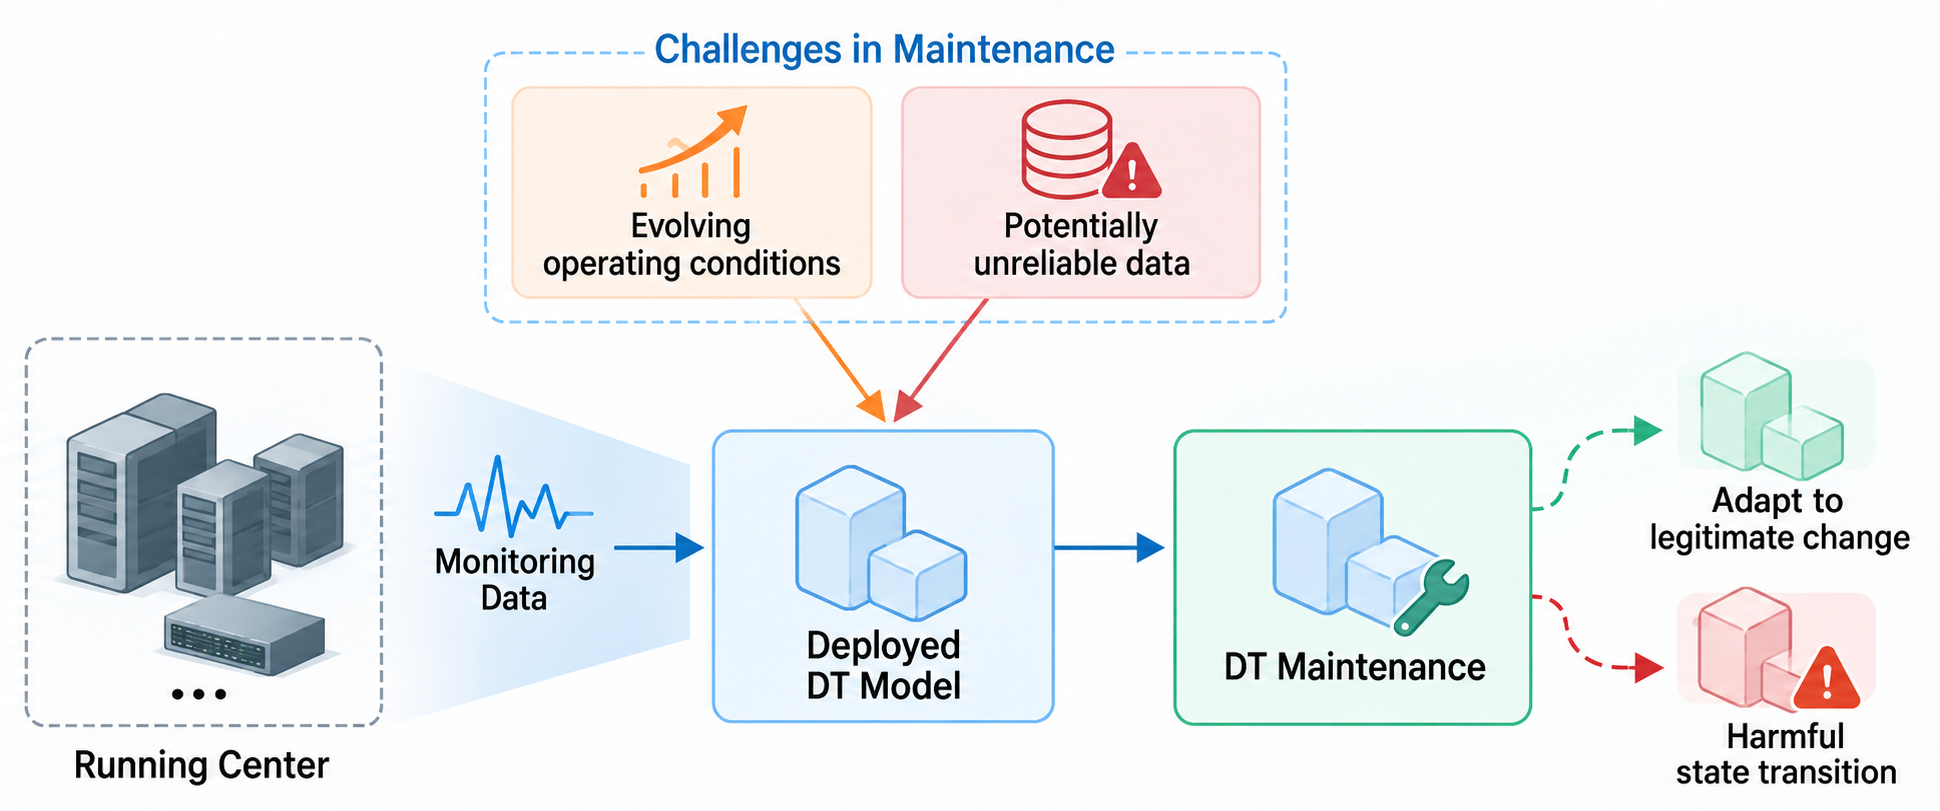
\includegraphics[width=0.88\textwidth]{fig1_problem_setting.pdf}
\caption{Problem setting for continual DT maintenance under evolving operating conditions and potentially unreliable monitoring data.}
\label{fig:problem-setting}
\end{figure}

Existing DT updating and synchronization methods maintain physical--virtual consistency as system conditions change \cite{li2024dtcl,rodriguez2023updating,amad2025calmdt}, while broader network-DT studies emphasize adaptive modeling and lifecycle synchronization \cite{qin2024dtnn,hakiri2024dtsurvey}. Continual-learning methods address sequential adaptation and knowledge retention, and reliability-oriented methods detect or mitigate unreliable observations before model modification. However, these lines of work do not explicitly treat post-adaptation state replacement as a separate deployment decision. When benign operating changes and unreliable observations coexist, successful adaptation on available maintenance data does not guarantee a beneficial deployed-state transition. The remaining challenge is therefore to make candidate-to-deployed state transitions reliable while retaining useful adaptation.

To address this challenge, we propose RAVM-DT, a verification-guided continual maintenance algorithm for deployed DT models. At each maintenance stage, RAVM-DT adapts the current model using update data to form a candidate, compares that candidate with the deployed state using paired recent and bounded historical verification evidence, and commits it only when both evidence criteria support replacement. Bounding the historical evidence horizon limits the influence of obsolete operating regimes while preserving temporally distinct evidence against harmful replacement.

The main contributions are as follows.
\begin{itemize}
    \item \textbf{State-transition formulation for continual DT maintenance.} We formulate maintenance under evolving and potentially unreliable monitoring data as repeated candidate-to-deployed state transitions, characterized by lifecycle loss, harmful-transition frequency, and harmful-transition downside.
    \item \textbf{Verification-guided selective state transition.} RAVM-DT separates candidate adaptation from deployment commitment and uses paired recent and bounded historical evidence to decide whether to commit or retain the current state.
    \item \textbf{Evaluation of the safety--utility--plasticity trade-off.} We evaluate the fixed RAVM-DT configuration under benign drift, multiple corruption patterns and severities, mechanism variants, model architectures, prediction horizons, maintenance cost, and an external production workload trace.
\end{itemize}

The remainder of this paper is organized as follows. Section~\ref{sec:related} reviews related work. Section~\ref{sec:problem} defines the problem, Section~\ref{sec:method} presents RAVM-DT, Section~\ref{sec:experiments} reports the evaluation, and Section~\ref{sec:conclusion} concludes the paper.

\section{Related Work}
\label{sec:related}

\subsection{Digital Twin Model Updating and Synchronization}
Digital-twin research has increasingly extended from one-time construction to post-deployment synchronization and updating. Li \emph{et al.} integrated continual learning into DT-enabled edge service provisioning \cite{li2024dtcl}, Rodriguez \emph{et al.} addressed data-quality control before automatic DT updating \cite{rodriguez2023updating}, and Amad \emph{et al.} explored continual updating with in-context large-language-model adaptation \cite{amad2025calmdt}. Recent DT-network surveys likewise identify adaptive modeling, synchronization, and AI-assisted lifecycle management as central challenges \cite{qin2024dtnn,hakiri2024dtsurvey}. These studies motivate continual maintenance, but primarily focus on how a model is updated or synchronized rather than whether an adapted candidate should replace the deployed state.

\subsection{Continual Adaptation under Evolving Conditions}
Continual learning studies sequential adaptation and the stability--plasticity trade-off \cite{parisi2019review,delange2022survey,wang2024clsurvey,son2025survey}, closely related to adaptation under concept drift \cite{gama2014drift}. Representative approaches preserve prior knowledge through parameter regularization \cite{kirkpatrick2017ewc}, distillation \cite{li2016lwf}, exemplar or episodic memory \cite{rebuffi2017icarl,lopezpaz2017gem,rolnick2019replay}, and importance-aware constraints \cite{aljundi2018mas}. Recent work has also analyzed forgetting and adaptation in continual regression settings \cite{ding2024forgetting}, while contaminated-stream methods explicitly address unreliable sequential data \cite{bang2022contaminated}. These methods improve adaptation, but an adapted model may still be unsuitable for deployment if the state transition itself is insufficiently supported.

\subsection{Reliable and Trustworthy DT Updating}
Reliable DT updating commonly emphasizes data-quality assessment, anomaly handling, and robust learning. Shen \emph{et al.} evaluate anomalous physical-twin data before trustworthy power-system DT updates \cite{shen2026trustworthy}. Robust estimation limits the influence of outlying observations \cite{huber1964robust}, while Byzantine-robust learning and poisoning research study unreliable or adversarial training information \cite{yin2018byzantine,biggio2012poisoning}. These directions improve the reliability of data or learning processes, but our focus is complementary: after a candidate has been adapted, should it replace the current deployed state when recent operating changes and potentially unreliable maintenance evidence coexist? RAVM-DT therefore targets the reliability of post-adaptation model-state transitions rather than adaptation alone.

\section{System Model and Problem Formulation}
\label{sec:problem}

\subsection{System Setting and Deployed DT Model}
We consider a DT platform that maintains center-specific models for a set of heterogeneous computing centers $\mathcal C$. For center $c\in\mathcal C$, let $a_c$ denote the architecture of its deployed DT model and let $\theta_{c,t}$ denote the model parameters after maintenance stage $t$. The deployed DT model state is represented as
\begin{equation}
M_{c,t}=(a_c,\theta_{c,t}),\qquad t=0,\ldots,T,
\label{eq:state}
\end{equation}
where $T$ is the number of maintenance stages.

The initial state $M_{c,0}$ is assumed to be valid and may be obtained by any model-instantiation procedure. We focus on parameter-state maintenance after deployment and keep $a_c$ fixed over the maintenance horizon. Repeated maintenance therefore produces the deployed-state sequence $M_{c,0}\rightarrow M_{c,1}\rightarrow\cdots\rightarrow M_{c,T}$.

\subsection{Operational Data and Model-State Transition}
At maintenance stage $t$, center $c$ provides newly matured operational data $\mathcal D^{\mathrm{maint}}_{c,t}$. The maintenance data are characterized from two complementary perspectives:
\begin{equation}
\mathcal D^{\mathrm{maint}}_{c,t}
=\mathcal D^{\mathrm{ben}}_{c,t}\uplus\mathcal D^{\mathrm{cor}}_{c,t},
\qquad
\mathcal D^{\mathrm{maint}}_{c,t}
=\mathcal D^{\mathrm{upd}}_{c,t}\uplus\mathcal D^{\mathrm{ver}}_{c,t},
\label{eq:data}
\end{equation}
where $\uplus$ denotes disjoint union. The first partition describes observation reliability: $\mathcal D^{\mathrm{ben}}_{c,t}$ contains legitimate operating observations, whereas $\mathcal D^{\mathrm{cor}}_{c,t}$ contains unreliable observations caused by measurement faults, stale data, communication faults, or manipulation. Their membership is unknown to the maintenance algorithm. The second partition specifies algorithmic roles. The update subset $\mathcal D^{\mathrm{upd}}_{c,t}$ is used to generate a candidate state, whereas the chronologically later verification subset $\mathcal D^{\mathrm{ver}}_{c,t}$ is excluded from candidate adaptation and provides evidence for the deployment decision. Either subset may contain unreliable observations.

For a prescribed candidate-adaptation operator $\mathcal A$, the candidate is
\begin{equation}
\widetilde{\theta}_{c,t}
=\mathcal A\!\left(\theta_{c,t-1},\mathcal D^{\mathrm{upd}}_{c,t}\right),
\qquad
\widetilde M_{c,t}=(a_c,\widetilde{\theta}_{c,t}).
\label{eq:candidate}
\end{equation}
Candidate generation does not by itself modify the deployed model. Let $u_{c,t}\in\{0,1\}$ denote the deployment decision, where $u_{c,t}=1$ commits the candidate and $u_{c,t}=0$ retains the current state. The deployed state after maintenance is
\begin{equation}
M_{c,t}=
\begin{cases}
\widetilde M_{c,t}, & u_{c,t}=1,\\
M_{c,t-1}, & u_{c,t}=0.
\end{cases}
\label{eq:commit-state}
\end{equation}
Thus, candidate adaptation and deployment commitment are distinct stages.

\subsection{Continual DT Model Maintenance Problem}
Let $\mathcal L(\mathcal D;M)$ denote the mean task loss of model state $M$ on dataset $\mathcal D$. Let $\mathcal D^{\mathrm{srv}}_{c,t}$ denote the service interval following the stage-$t$ deployment decision. These data are unavailable when $u_{c,t}$ is determined and are used only to evaluate the subsequent consequence. Define
\begin{equation}
\Delta_{c,t}
=\mathcal L\!\left(\mathcal D^{\mathrm{srv}}_{c,t};\widetilde M_{c,t}\right)
-\mathcal L\!\left(\mathcal D^{\mathrm{srv}}_{c,t};M_{c,t-1}\right).
\label{eq:delta}
\end{equation}
A negative $\Delta_{c,t}$ indicates that the candidate would improve subsequent service performance relative to retaining the current state, whereas a positive value indicates degradation. A harmful state transition therefore occurs when the candidate is committed and $\Delta_{c,t}>0$.

For the prescribed candidate-adaptation operator $\mathcal A$, the ideal deployment-decision problem is
\begin{equation}
\begin{aligned}
\min_{\{u_{c,t}\}}\quad
&\frac{1}{|\mathcal C|T}
\sum_{c\in\mathcal C}\sum_{t=1}^{T}
\mathcal L\!\left(\mathcal D^{\mathrm{srv}}_{c,t};M_{c,t}\right)\\
\mathrm{s.t.}\quad
&\frac{1}{|\mathcal C|T}
\sum_{c\in\mathcal C}\sum_{t=1}^{T}
 u_{c,t}\mathbf 1[\Delta_{c,t}>0]\leq \rho,\\
&\frac{1}{|\mathcal C|T}
\sum_{c\in\mathcal C}\sum_{t=1}^{T}
 u_{c,t}[\Delta_{c,t}]_{+}\leq \epsilon,
\end{aligned}
\label{eq:ideal-problem}
\end{equation}
where $|\mathcal C|$ is the number of computing centers, $\mathbf 1[\cdot]$ is the indicator function, $[z]_{+}=\max(z,0)$, $\rho\in[0,1]$ is the tolerated harmful-transition frequency, and $\epsilon\geq0$ is the tolerated average harmful-transition downside.

Equation~\eqref{eq:ideal-problem} defines an ideal lifecycle objective and risk criteria rather than an online guarantee. At maintenance time, $\mathcal D^{\mathrm{srv}}_{c,t}$ and hence $\Delta_{c,t}$ are unavailable. The practical problem is therefore to determine $u_{c,t}$ using only information available before the subsequent service interval, while maintaining lifecycle utility and limiting harmful deployed-state transitions.

\section{Proposed RAVM-DT Algorithm}
\label{sec:method}

\subsection{Overview}
RAVM-DT solves the decision problem in Section~\ref{sec:problem} by separating candidate adaptation from deployment commitment. At stage $t$, update data produce one candidate state, recent and bounded historical verification evidence compare that candidate with the current deployed state, and a selective decision either commits the candidate or retains the current state. Current verification data enter the historical buffer only after the decision. Figure~\ref{fig:overview} summarizes this workflow.

\begin{figure}[t]
\centering
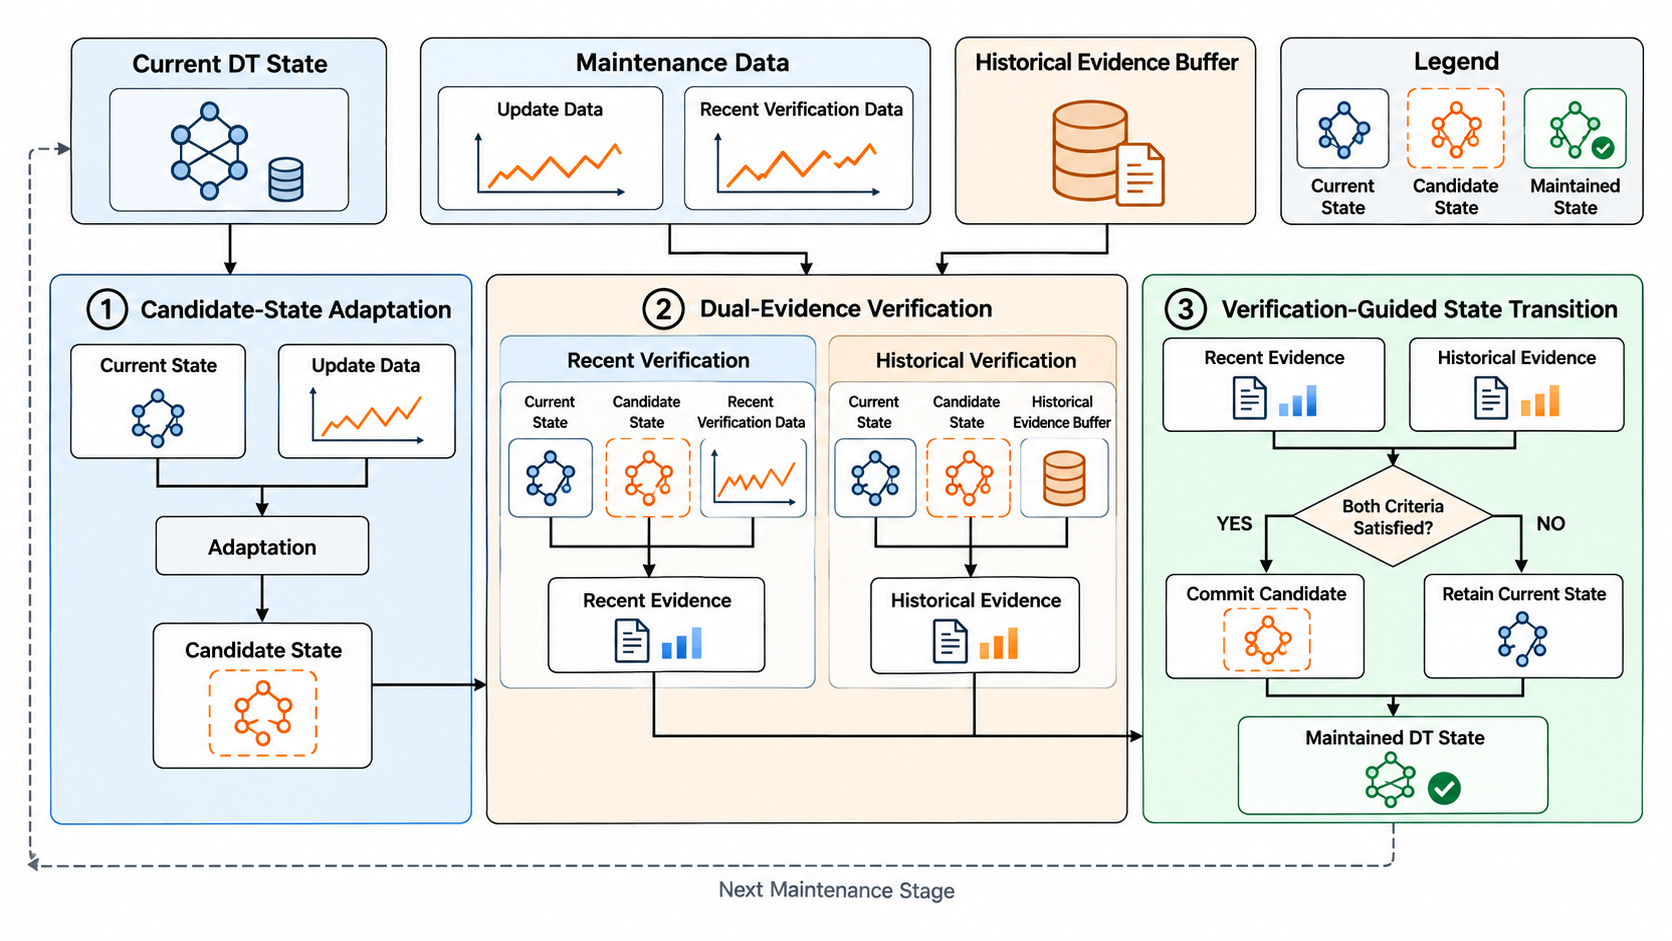
\includegraphics[width=0.92\textwidth]{fig2_ravm_dt_framework.pdf}
\caption{Overview of RAVM-DT. A single candidate state is adapted from the current DT state using update data, evaluated through recent and bounded historical evidence, and committed only when both criteria support replacement; otherwise, the current state is retained as the maintained DT state.}
\label{fig:overview}
\end{figure}

\subsection{Candidate-State Adaptation}
At each stage, the candidate starts as an isolated copy of the current deployed state and is optimized only with update data. Let $\mathcal B^{(s)}_{c,t}\subseteq\mathcal D^{\mathrm{upd}}_{c,t}$ denote the update mini-batch used at step $s$. A gradient-based realization of the candidate-adaptation operator in Eq.~\eqref{eq:candidate} is
\begin{equation}
\begin{aligned}
\theta^{(0)}_{c,t}&=\theta_{c,t-1},\\
\theta^{(s+1)}_{c,t}&=\theta^{(s)}_{c,t}-\eta\nabla_{\theta}\mathcal L\!\left(\mathcal B^{(s)}_{c,t};(a_c,\theta^{(s)}_{c,t})\right),\quad s=0,\ldots,S-1,\\
\widetilde{\theta}_{c,t}&=\theta^{(S)}_{c,t},\qquad \widetilde M_{c,t}=(a_c,\widetilde{\theta}_{c,t}),
\end{aligned}
\label{eq:adaptation}
\end{equation}
where $S$ is the stage-level adaptation budget and $\eta$ the learning rate. The complete update subset defines the sampling pool, while $\mathcal D^{\mathrm{ver}}_{c,t}$ is excluded from parameter updates and the deployed state is unchanged until commitment.

\subsection{Dual-Evidence Verification}
Each verification collection is partitioned chronologically into $B$ block units; target windows belong to one block, although their input contexts may overlap because of sliding-window construction. Let $\mathcal E^{\mathrm{rec}}_{c,t}=\mathcal D^{\mathrm{ver}}_{c,t}$ and let $\mathcal E^{\mathrm{hist}}_{c,t-1}$ denote blocks retained in a bounded historical buffer. Before the first online stage, $\mathcal H_{c,0}$ is initialized from target-specific pre-maintenance verification evidence. For $q\in\{\mathrm{rec},\mathrm{hist}\}$ and chronological block $\mathcal E^{q}_{c,t,j}$, RAVM-DT evaluates the candidate and current state on the same block:
\begin{equation}
d^{q}_{c,t,j}=\mathcal L\!\left(\mathcal E^{q}_{c,t,j};\widetilde M_{c,t}\right)-\mathcal L\!\left(\mathcal E^{q}_{c,t,j};M_{c,t-1}\right).
\label{eq:paired}
\end{equation}
Negative values favor the candidate. The paired differences are summarized by
\begin{equation}
\begin{aligned}
m^{q}_{c,t}&=\operatorname{median}_{j}d^{q}_{c,t,j},\\
r^{q}_{c,t}&=\operatorname{median}_{j}\left|d^{q}_{c,t,j}-m^{q}_{c,t}\right|,\\
U^{q}_{c,t}&=m^{q}_{c,t}+\kappa_q r^{q}_{c,t},\qquad q\in\{\mathrm{rec},\mathrm{hist}\},
\end{aligned}
\label{eq:evidence-score}
\end{equation}
where $\kappa_q\geq0$ controls the penalty for disagreement among verification blocks. $U^{q}_{c,t}$ is a robust conservative evidence score, not a formal statistical confidence bound.

\subsection{Verification-Guided State Transition}
Let $\delta_{\mathrm{imp}}\geq0$ be the required recent improvement and $\delta_{\mathrm{ret}}\geq0$ the tolerated historical degradation. The deployment decision is
\begin{equation}
u_{c,t}=\begin{cases}
1, & U^{\mathrm{rec}}_{c,t}\leq-\delta_{\mathrm{imp}}\ \text{and}\ U^{\mathrm{hist}}_{c,t}\leq\delta_{\mathrm{ret}},\\
0, & \text{otherwise}.
\end{cases}
\label{eq:commit-rule}
\end{equation}
Thus, recent evidence requires adaptation benefit while historical evidence limits degradation of recently retained behavior. The historical buffer has capacity $C_{\mathrm{hist}}$; after the stage-$t$ decision, current verification blocks are appended and the oldest blocks are evicted if necessary. This ordering prevents current verification data from influencing their own decision through the historical branch and limits the effect of obsolete regimes.

\begin{Algorithm}[RAVM-DT Maintenance for Center $c$ at Stage $t$]
\label{alg:method}
\normalfont\small
\setlength{\emergencystretch}{1.5em}
\begin{enumerate}[label=\arabic*.,leftmargin=2.2em,labelwidth=1.2em,labelsep=0.4em,itemsep=0pt,topsep=1pt]
\item \textbf{Input:} $M_{c,t-1}$, $\mathcal D^{\mathrm{upd}}_{c,t}$, $\mathcal D^{\mathrm{ver}}_{c,t}$, historical buffer $\mathcal H_{c,t-1}$, and method parameters.
\item Adapt on $\mathcal D^{\mathrm{upd}}_{c,t}$ using Eq.~\eqref{eq:adaptation} to obtain $\widetilde M_{c,t}$.
\item Form recent and historical evidence and compute Eqs.~\eqref{eq:paired}--\eqref{eq:evidence-score}.
\item Determine $u_{c,t}$ by Eq.~\eqref{eq:commit-rule} and update $M_{c,t}$ by Eq.~\eqref{eq:commit-state}.
\item \textbf{After the decision}, append current verification blocks to $\mathcal H_{c,t-1}$ and evict the oldest blocks if required.
\item \textbf{Return:} $M_{c,t}$ and the updated buffer $\mathcal H_{c,t}$.
\end{enumerate}
\end{Algorithm}

\subsection{Decision-Parameter Calibration}
Let $\gamma\in\Gamma$ denote a candidate decision-parameter configuration. On calibration data disjoint from final evaluation, let $\widehat{\mathcal R}(\gamma)$, $\widehat{\mathcal H}(\gamma)$, and $\widehat{\mathcal S}(\gamma)$ denote empirical lifecycle loss, harmful-transition frequency, and harmful-transition downside. We select
\begin{equation}
\gamma^{*}\in\arg\min_{\gamma\in\Gamma}\widehat{\mathcal R}(\gamma)
\quad\mathrm{s.t.}\quad
\widehat{\mathcal H}(\gamma)\leq\rho,\qquad
\widehat{\mathcal S}(\gamma)\leq\epsilon.
\label{eq:calibration}
\end{equation}
The selected configuration is fixed before final evaluation. Equation~\eqref{eq:calibration} is an offline calibration rule; online decisions still use only information available before the subsequent service interval.

\section{Experimental Evaluation}
\label{sec:experiments}
\subsection{Experimental Setup}
\subsubsection{Benchmark and Lifecycle Protocol}
Workload prediction is used as the maintenance task, following its role in proactive cloud/resource management \cite{kim2024workload,zuo2025workload,zhao2025mscnet,feng2025workloadsurvey}. Method development, decision calibration, and final evaluation use disjoint center pools; the final pool contains 30 centers, three fixed model seeds per center, and 24 chronological stages. For each target center, the initial deployed model is obtained by source pretraining followed by 50-step target warm-up adaptation on the first 800 raw observations. A disjoint 200-observation pre-maintenance interval initializes six historical verification blocks. Each stage then follows a raw-first causal split of 400 update, 240 verification, and 400 service observations; windows are formed separately within each role, giving 304/144/304 windows for $L=96,H=1$. The preceding service interval becomes the next stage's update interval only after its labels mature. The main predictor is a one-layer GRU-32; architecture/horizon generality is examined in Section~\ref{sec:sensitivity}.

\subsubsection{Method Configuration and Calibration}
Method structure is fixed on the development pool and decision parameters are calibrated on a disjoint pool before final evaluation. Each verification subset is divided into six chronological blocks, and the 12-block history is updated by FIFO truncation only after the current decision. The decision search uses $\kappa_{\mathrm{rec}},\kappa_{\mathrm{hist}}\in\{0,0.5,1.0,1.5\}$; among configurations satisfying the absolute harmful-transition and downside criteria on mixed, persistent-bias, and replay calibration settings, lifecycle MSE is minimized with a deterministic tie-break. Table~\ref{tab:configuration} reports the fixed configuration.

\begin{table}[t]
\centering
\caption{Main Experimental Configuration}
\label{tab:configuration}
\scriptsize
\begin{tabular}{lll}
\toprule
Category & Item & Setting \\
\midrule
Lifecycle & Centers / seeds / stages & 30 / 3 / 24 \\
Predictor & Architecture / input / horizon & GRU-32 / $L=96$ / $H=1$ \\
Adaptation & Optimizer / loss / updates & SGD / MSE / 50 \\
 & Learning rate / clipping & 0.01 / 1.0 \\
 & Batch / sampling / weight decay & 64 / replacement / 0 \\
Verification & Blocks per stage / history capacity & 6 / 12 blocks \\
 & $\kappa_{\mathrm{rec}},\kappa_{\mathrm{hist}}$ & $0,\ 0.5$ \\
Commitment & $\delta_{\mathrm{imp}},\delta_{\mathrm{ret}}$ & $2.8018\!\times\!10^{-5},\ 0$ \\
Risk criteria & $\rho,\epsilon$ & $0.05,\ 5.6036\!\times\!10^{-5}$ \\
Statistics & Unit / bootstrap & Center / 4000 repetitions \\
 & Model / attack / bootstrap seeds & 7311--7313 / 9417 / 2904 \\
Hardware & GPU & RTX 3060 Laptop GPU \\
\bottomrule
\end{tabular}
\end{table}

\subsubsection{Conditions, Baselines, Metrics, and Statistics}
The four benign regimes apply a deterministic scalar workload shift: stationary remains unchanged, gradual ramps from 0 to 0.8, abrupt switches to 0.8 at the stage-9 verification boundary, and recurring alternates between shifted and unshifted intervals. The mixed condition overlays telemetry corruption with nominal fraction $\alpha=0.10$ on each center's base regime. Each role segment is divided into ten temporal strata and $\lfloor n_s\alpha\rfloor$ positions per stratum are corrupted; mixed corruption cycles random noise, stage-persistent bias, bursts, and replay, while service data remain clean. Persistent-bias, replay, and additional $\alpha$ values are examined in Section~\ref{sec:severity}.

We compare RAVM-DT with Always-FT, experience replay (ER) \cite{rolnick2019replay}, elastic weight consolidation (EWC) \cite{kirkpatrick2017ewc}, Huber-loss fine-tuning (Huber-FT) \cite{huber1964robust}, ValidationCommit, and Frozen. Active methods share the 50-step adaptation budget; ER uses FIFO raw replay, EWC uses $\lambda=10$ with Fisher EMA $\gamma=0.9$, and Huber-FT uses $\delta=0.1$. ValidationCommit uses the whole-verification mean candidate--current loss difference with a calibrated threshold; its calibration triggered the retain-all fallback, yielding zero final-pool commitments. Lifecycle MSE is the primary utility metric; transition safety is measured by harmful-transition frequency and average downside, with commit rate and beneficial-commit recall characterizing adaptation. Centers are the statistical units: seeds are averaged within center and paired 95\% intervals use 4000 center-cluster bootstrap repetitions. For all methods, service data are excluded from candidate adaptation and deployment commitment.

\subsection{Overall Lifecycle Maintenance Performance}
\label{sec:overall}
\begin{figure}[t]
\centering
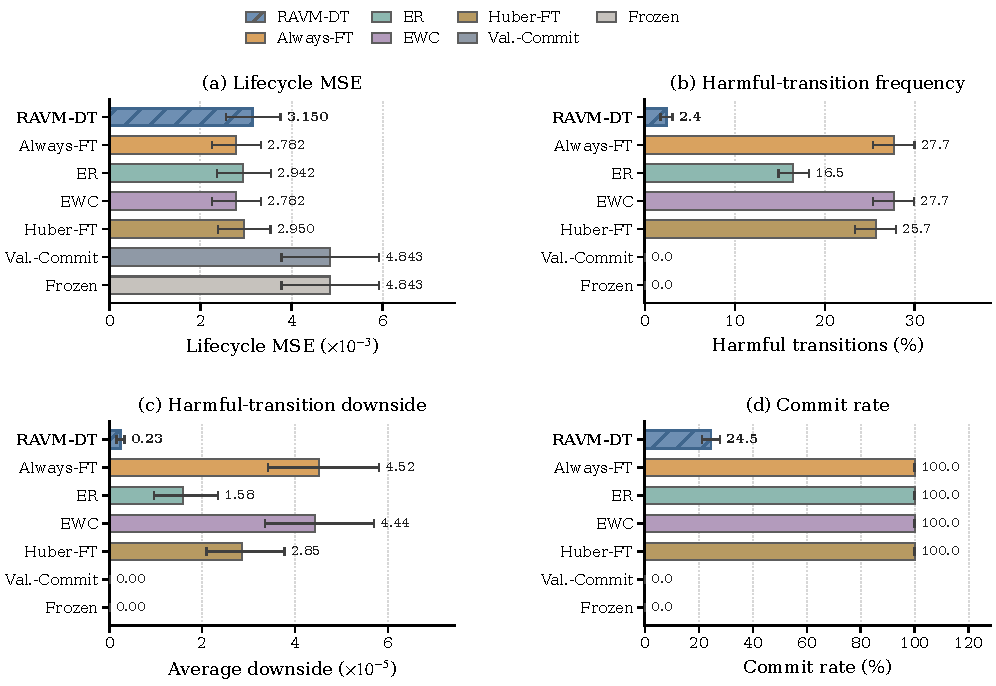
\includegraphics[width=0.80\textwidth]{fig3_overall_baseline.pdf}
\caption{Overall lifecycle performance over the five primary conditions: (a) MSE, (b) harmful-transition frequency, (c) average harmful downside, and (d) commit rate. Error bars denote 95\% center-cluster bootstrap intervals.}
\label{fig:overall}
\end{figure}

Figure~\ref{fig:overall} shows the central safety--utility--plasticity trade-off. Active always-update baselines achieve lower MSE, whereas RAVM-DT incurs about 6.8\%--13.2\% higher MSE but reduces harmful-transition frequency by about 85.5\%--91.4\% and harmful downside by 85.3\%--94.9\%. ValidationCommit makes no final-pool commitments and therefore follows Frozen; relative to this no-update reference, RAVM-DT lowers MSE by about 34.9\% while committing roughly one quarter of candidate states. Thus, its safety gain is not obtained by disabling adaptation.

\subsection{Robustness to Unreliable Monitoring Data}
\label{sec:severity}
\begin{figure}[t]
\centering
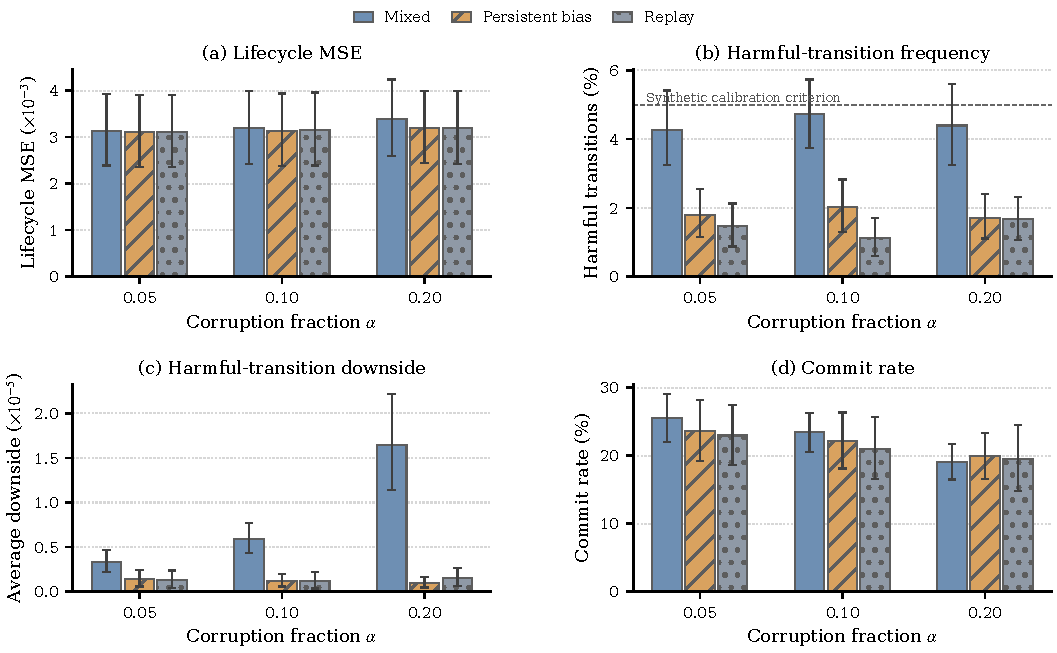
\includegraphics[width=0.74\textwidth]{fig4_corruption_severity.pdf}
\caption{Robustness across corruption severities. Mixed corruption affects update and verification data; persistent bias and replay target verification evidence. Panels report MSE, harmful-transition frequency, harmful downside, and commit rate for $\alpha\in\{0.05,0.10,0.20\}$.}
\label{fig:severity}
\end{figure}

Across the nine tested corruption--severity combinations in Fig.~\ref{fig:severity}, harmful-transition frequency remains below the 5\% synthetic-domain calibration criterion. Mixed corruption produces the clearest utility/downside deterioration as $\alpha$ increases, while commit rates decline across all three corruption types. The safety metric is not monotone in nominal corruption fraction, so the result is interpreted as robustness within the evaluated range rather than a general severity law.

\subsection{Adaptation under Benign Operating Evolution}
\label{sec:benign}
\begin{figure}[t]
\centering
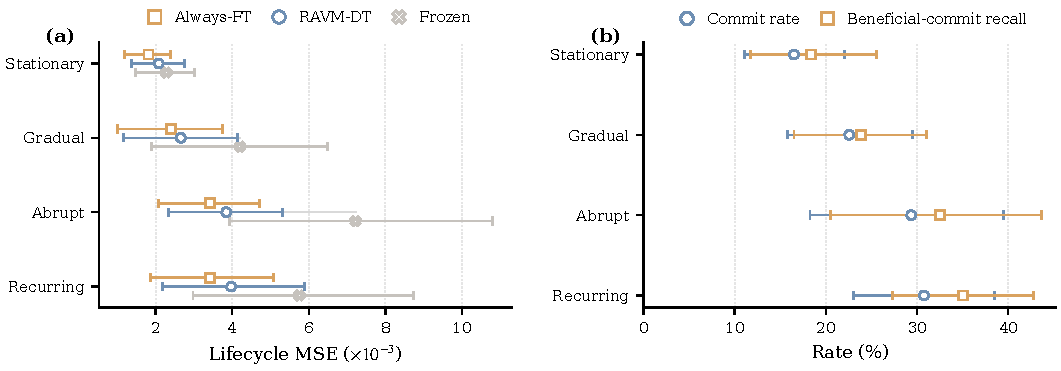
\includegraphics[width=0.70\textwidth]{fig5_benign_evolution.pdf}
\caption{Benign operating evolution: (a) lifecycle MSE for RAVM-DT, Always-FT, and Frozen; (b) RAVM-DT commit rate and beneficial-commit recall. Error bars denote 95\% center-cluster bootstrap intervals.}
\label{fig:benign}
\end{figure}

Always-FT remains the lowest-MSE reference, but RAVM-DT substantially outperforms Frozen under gradual, abrupt, and recurring drift. Its commit rate and beneficial-commit recall are higher under gradual, abrupt, and recurring drift than under stationary conditions, while harmful-transition frequency remains about 1.0\%--2.6\% across the four benign regimes. The method therefore retains selective plasticity at a measurable utility cost relative to unrestricted adaptation.

\subsection{Mechanism Analysis}
\label{sec:mechanism}
\begin{figure}[t]
\centering
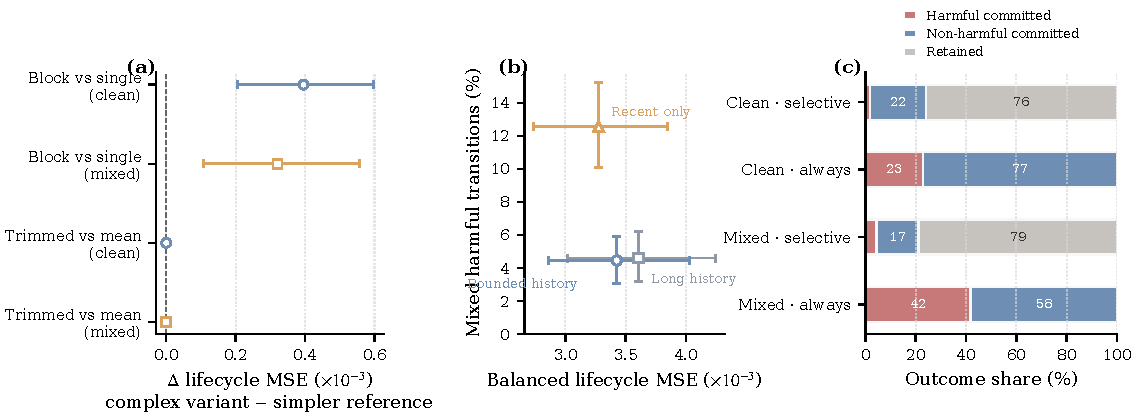
\includegraphics[width=0.78\textwidth]{fig6_mechanism_analysis.pdf}
\caption{Mechanism analysis on the development pool: (a) paired MSE effects of additional candidate-side complexity, (b) utility--risk trade-off of recent-only, long-history, and bounded-history verification, and (c) deployment outcomes for selective and always-commit variants.}
\label{fig:mechanism}
\end{figure}

Figure~\ref{fig:mechanism}(a) provides no evidence that the tested candidate-side complexity variants---blockwise construction or trimmed state-delta aggregation---improve the final maintenance outcome, supporting the simpler single-path candidate. Figure~\ref{fig:mechanism}(b) shows that recent-only verification is more plastic but reaches about 12.6\% harmful transitions under mixed corruption; adding history sharply reduces this exposure, while bounding the retained history recovers utility relative to a longer history. Finally, Fig.~\ref{fig:mechanism}(c) shows that selective commitment strongly reduces harmful replacement at the cost of retaining more candidates. Together, these results support simple candidate adaptation followed by bounded temporal verification and selective deployment control.

\subsection{Sensitivity, Generality, and Maintenance Cost}
\label{sec:sensitivity}
\begin{figure}[t]
\centering
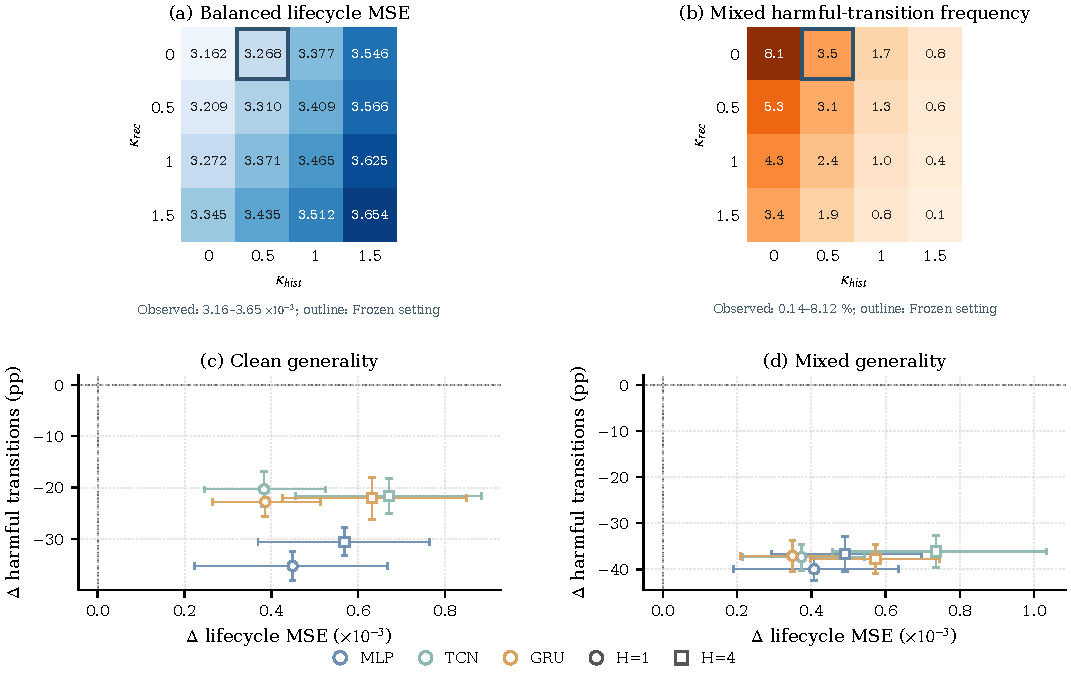
\includegraphics[width=0.72\textwidth]{fig7_sensitivity_generality.pdf}
\caption{Sensitivity and generality of RAVM-DT. Panels (a)--(b) show the predefined $\kappa_{\mathrm{rec}}\times\kappa_{\mathrm{hist}}$ grid; the outlined cell is the fixed setting $(0,0.5)$. Panels (c)--(d) show clean and mixed effects, computed as RAVM-DT minus Always-FT, across MLP, TCN, and GRU with $H\in\{1,4\}$.}
\label{fig:sensitivity}
\end{figure}

The sensitivity grid in Fig.~\ref{fig:sensitivity}(a)--(b) exposes an explicit utility--risk trade-off; the fixed setting lies on the observed frontier but is not claimed to be universally optimal. Without architecture- or horizon-specific retuning, the expected qualitative ordering is retained in all 12 tested architecture--horizon--condition cells: RAVM-DT pays a positive MSE cost relative to Always-FT while reducing harmful-transition frequency. This supports consistency across the tested settings, not architecture-invariant performance.

\begin{table}[t]
\centering
\caption{Measured Maintenance Cost in the Final Benchmark}
\label{tab:cost}
\scriptsize
\begin{tabular}{lrrr}
\toprule
Method & Runtime/stage (s) & Peak GPU (MB) & Buffer (kB) \\
\midrule
RAVM-DT & 0.185 & 55.7 & 155.5 \\
Always-FT & 0.250 & 55.6 & 0 \\
ER & 0.262 & 98.3 & 302.4 \\
EWC & 0.504 & 58.3 & 44.8 \\
Huber-FT & 0.250 & 55.6 & 0 \\
ValidationCommit & 0.252 & 67.7 & 0 \\
Frozen & 0.004 & 25.5 & 0 \\
\bottomrule
\end{tabular}
\end{table}

Table~\ref{tab:cost} shows that RAVM-DT requires about 0.185~s per maintenance stage, 55.7~MB peak GPU memory, and a 155.5~kB persistent buffer on the evaluated platform. Timing covers update construction, adaptation, verification, commitment, and maintenance bookkeeping, but excludes subsequent service evaluation and file I/O. Its runtime is of the same order as the adaptive baselines; these measurements characterize the implementation rather than a general latency guarantee.

\subsection{External Production-Trace Evaluation}
\label{sec:external}
\begin{figure}[t]
\centering
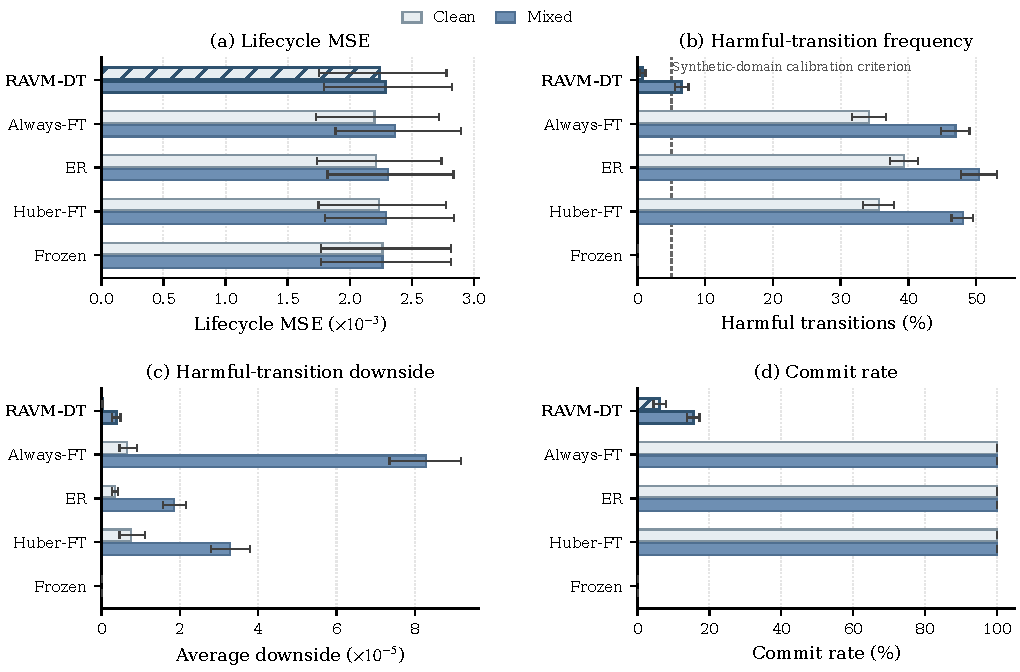
\includegraphics[width=0.68\textwidth]{fig8_alibaba_external.pdf}
\caption{External Alibaba-trace evaluation under clean and mixed corruption. Panels report (a) lifecycle MSE, (b) harmful-transition frequency, (c) harmful downside, and (d) commit rate. The 5\% line in (b) is the synthetic-domain calibration criterion.}
\label{fig:external}
\end{figure}

We finally evaluate the fixed configuration on the reconstructed 40-machine Alibaba Cluster Trace split \cite{alibaba2018trace}, without target-domain recalibration. For each selected machine, the first 17,000 valid timestamp-sorted observations are retained without interpolation; seven telemetry values are represented with value/mask channels and processed by the same causal lifecycle protocol. Under clean workloads, RAVM-DT is close to the active baselines in MSE while showing much lower harmful-transition exposure. Under mixed corruption, it remains selectively active and strongly reduces harmful transitions/downside relative to active baselines, but its harmful-transition frequency reaches 6.49\%, above the 5\% synthetic-domain calibration criterion, and its MSE is slightly higher than Frozen. The result therefore supports qualitative transfer of selective state-transition control, while showing that the exact risk operating point can be domain dependent.

\section{Conclusion}
\label{sec:conclusion}
This paper presented RAVM-DT for continual maintenance of deployed DT models under evolving and potentially unreliable monitoring data. By separating candidate adaptation from deployment commitment, RAVM-DT uses paired recent and bounded historical verification evidence to decide whether an adapted candidate should replace the current state. Across the five primary lifecycle conditions, it reduces harmful-transition frequency by about 85.5\%--91.4\% and harmful downside by 85.3\%--94.9\% relative to active adaptation baselines, at a 6.8\%--13.2\% MSE increase; relative to Frozen, it lowers MSE by about 34.9\% while retaining nonzero adaptation. Mechanism, benign-drift, and architecture/horizon results support the intended selective-transition behavior rather than a retain-all policy. On Alibaba workloads, the same qualitative safety control transfers, but the 6.49\% mixed-condition harmful-transition frequency exceeds the 5\% synthetic calibration criterion, indicating domain-dependent risk calibration. Current evidence is empirical and limited to workload prediction on one controlled benchmark and one external trace; future work will study calibration under domain shift, additional DT tasks/platforms, and mechanisms that improve adaptation without sacrificing transition safety.


% Mandatory TSP statements.
\acknowledgement{During the preparation of this manuscript, the authors used OpenAI ChatGPT (GPT-5.6 Sol) for language polishing and editorial revision. The authors subsequently reviewed and revised the relevant content and accept full responsibility for the article.}
\funding{This work was supported in part by the Major Science and Technology Special Project of Qinghai Office of Science and Technology, China, under Grant No. 2024-GX-A3.}
\authorcontributions{The authors confirm contribution to the paper as follows: conceptualization, Jianyong Wang; methodology, Jianyong Wang; software, Jianyong Wang; validation, Jianyong Wang; formal analysis, Jianyong Wang; investigation, Jianyong Wang; data curation, Jianyong Wang; visualization, Jianyong Wang; writing---original draft preparation, Jianyong Wang; writing---review and editing, Jie Liu, Yubo Dong, Tengyu Gai and Fengbiao Zan. All authors reviewed and approved the final version of the manuscript.}
\availabilityofdataandmaterials{The implementation code, experimental configurations, and processed results supporting the findings of this study are available from the corresponding author upon reasonable request. The Alibaba Cluster Trace used for external evaluation is a publicly available third-party dataset and should be obtained from the original provider; it is not redistributed with this article.}
\ethicsapproval{Not applicable. This study does not involve human participants or animals.}
\conflictsofinterest{The authors declare no conflicts of interest. The funder had no role in the design of the study; in the collection, analyses, or interpretation of data; in the writing of the manuscript; or in the decision to publish the results.}

\reftitle{References}
\bibliography{bibliography/references}

\end{document}
